\documentclass[acmtog]{acmart}
\usepackage{graphicx}
\usepackage{subfigure}
\usepackage{natbib}
\usepackage{listings}
\usepackage{bm}
\usepackage{amsmath}

\definecolor{blve}{rgb}{0.3372549 , 0.61176471, 0.83921569}
\definecolor{gr33n}{rgb}{0.29019608, 0.7372549, 0.64705882}
\makeatletter
\lst@InstallKeywords k{class}{classstyle}\slshape{classstyle}{}ld
\makeatother
\lstset{language=C++,
	basicstyle=\ttfamily,
	keywordstyle=\radiance{blve}\ttfamily,
	stringstyle=\radiance{red}\ttfamily,
	commentstyle=\radiance{magenta}\ttfamily,
	morecomment=[l][\radiance{magenta}]{\#},
	classstyle = \bfseries\radiance{gr33n},
	tabsize=2
}
\lstset{basicstyle=\ttfamily}

% Title portion
\title{CS171 Final Project: {Ray Tracing NURBS surfaces}}

\author{Group Number:\quad 10 \\
Member 1:\quad Xiyue Peng\\
Member 2:\quad Luojia Hu
}

% Document starts
\begin{document}
\maketitle

\vspace*{2 ex}

\section{Introduction}

In this project, we implemented an algorithm for directly ray tracing NURBS surfaces without generating mesh first and ray tracing the mesh. % By ray tracing NURBS directly, we can avoid the dilemma that we have to generate a fine enough mesh while maintaining a reasonable memory usage and computation time. 


\section{Implementation Details}

In this section, we will discuss the NURBS surface representation and the `direct' ray tracing NURBS algorithm we implemented. In short, we first flatten the control points to get a refined control mesh, and then generate a BVH from it. During ray tracing step, we use the Newton-Rhapson method to find intersection with surface patches. Finally we integrated it into the global illumination ray tracing framework to get the result. 

\subsection{NURBS Surface Representation}

% 这里介绍一下NURBS

A \textbf{Non-Uniform Rational B-spline Surface}, or \textbf{NURBS}, is a generalization of B-spline surfaces. A NURBS curve is defined by a set of \textbf{control points}, along with a weight for each control point called \textbf{knot vector} and a \textbf{knot vector} used for fine-tuning the shape. 

The \textbf{control points} are the vertices of the surface, and the weights are the weights of the vertices. 

The knots or \textbf{knot vector} is a list of $(\mathrm{degree}+N-1)$ numbers where $N$ is the number of control points. It should be an non-decreasing sequence, and the number of duplicate values cannot be larger than the degree. For example, for a degree 3 NURBS curve with 11 control points, $0,0,0,1,2,2,2,3,7,7,9,9,9$ is an acceptable knot vector. The number of times a knot value is duplicated is called the knot's \textbf{multiplicity}. 

The surface is defined by the following equation: 

\begin{equation}
	\label{eq:1} % TODO: 公式没改完
	\mathbf{S}^w(u,v) = \sum_{i=0}^{M-1} \sum_{j=0}^{N-1} \mathbf{P}_{i,j}^w w_{i,j} B_{i,p}(u) B_{j,q}(v) P_{i,j}
\end{equation}

where $\mathbf{P}$ are the control points of the $M\times N$ control mesh, which has basis functions $B_{j,k_u}, B_{i, k_v}$ of orders $k_u$ and $k_v$ defined over knot vectors.

where $B_{i,p}(u)$ is the $i$th B-spline basis function of degree $p$ at $u$, $P_{i,j}$ is the $i$th control point of the $j$th row, and $w_{i,j}$ is the weight of the $i$th control point of the $j$th row. The degree of the surface is $p$ in the $u$ direction and $q$ in the $v$ direction. The surface is defined on the domain $[u_{0}, u_{n+p+1}] \times [v_{0}, v_{m+q+1}]$, where $u_{0} = v_{0} = 0$ and $u_{n+p+1} = v_{m+q+1} = 1$. 
% The knot vectors are defined as follows:

% \begin{equation}
% \label{eq:2}
% u_{i} = \begin{cases}
% 0 & \text{if } i \leq p \\
% \frac{i-p}{n+1} & \text{if } p < i \leq n \\
% 1 & \text{if } i > n
% \end{cases}
% \end{equation}

% \begin{equation}
% \label{eq:3}
% v_{j} = \begin{cases}
% 0 & \text{if } j \leq q \\
% \frac{j-q}{m+1} & \text{if } q < j \leq m \\
% 1 & \text{if } j > m
% \end{cases}
% \end{equation}

% where $n$ and $m$ are the number of control points in the $u$ and $v$ directions, respectively. The knot vectors are non-decreasing, and the knot vectors are clamped at the ends. The knot vectors are also called \textbf{clamped knot vectors}.

\subsection{Preprocessing}

% TODO: 这里介绍一下如何用NURBS创建BVH (描述细分过程等等)
In the reprocessing step, 
similar to what we did in ray tracing a Triangle Mesh, we need to create a BVH for the NURBS surface. The difference is that we need to subdivide the original NURBS surface's control points into a \textbf{refined control mesh}, instead of calculating triangle mesh coordinates directly. 

The following figure is an intuitive illustration of the NURBS curve's BVH. 

\begin{figure}[H]
	\centering
	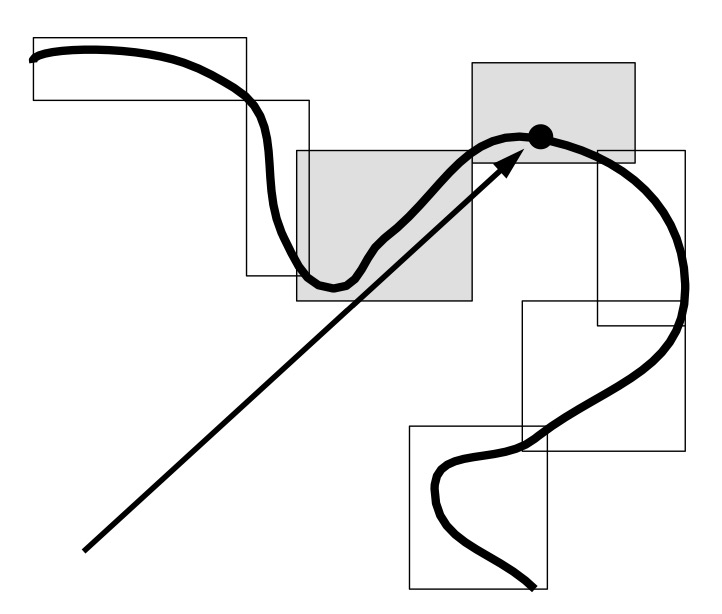
\includegraphics[width=0.3\textwidth]{pictures/bvh.jpg}
	\caption{A NURBS curve with a series of axis-aligned bounding boxes (AABB) generated. A ray is tested for intersection with AABBs.}
\end{figure}

Flattening TODO:

In order for an accurate initial guess during intersection test, we need to refine, or subdivide the control mesh into a finer one. We use a curvature-based refinement of knot vectors. We need to ensure that the result meets some flatness criteria, in order for generating an accurate bounding box. The number of knots going to be added is based on the curvature of the surface (?). 

\[
	n = C \cdot \max_{t_i, t_{i+1}} \{ \mathrm{curvature}(\mathbf{c(t)}) \} \cdot \mathrm{arclen}(\mathbf{c}(t))_{[t_i, t_{i+1})}^{3/2}	
\]

where $C$ is a fineness constant parameter to be adjusted. 

The arc length of $\mathbf{c}$ is given by \[
	\int_{t_i}^{t_{i+1}} |\mathbf{c}'(t) | dt 
	= \mathrm{avg}_{[t_i, t_{i+1})} \{ |\mathbf{c}'(t)| \} \cdot (t_{i+1} - t_i)	
\]

The curvature is defined as \[\begin{aligned}
	\mathrm{curvature}(\mathbf{c}(t)) &= 
	\frac{|\mathbf{c}''(t) \times \mathbf{c}'(t)|}{|\mathbf{c}'(t)|^3}\\
	&= \frac{|\mathbf{c}''(t)| |\sin(\theta)|}{|\mathbf{c}'(t)|^2}\\
	&\leq \frac{|\mathbf{c}''(t)|}{|\mathbf{c}'(t)|^2}
\end{aligned}\]

We assume the curvature is $\frac{|\mathbf{c}''(t)|}{|\mathbf{c}'(t)|^2}$ since in this way the curvature estimate will be higher, meaning we will refine slightly higher rather than not enough. 

BVH TODO:

After generating the refined control mesh, we build a bounding volume hierarchy, or BVH. The leaf nodes are 

\subsection{Ray Tracing NURBS Directly}

\subsubsection{Transform ray equation}
% 我们需要把一条ray从o+td的形式,写成两个平面的交集的形式
\ 

Recall that a ray can be represented by $\mathbf{r} = \mathbf{o} + t \mathbf{d}$, where $\mathbf{o}$ is the ray's origin and $\mathbf{d}$ is the normalized direction. However in order for ray intersection test for NURBS, we will rewrite the ray $\mathbf{r}$ as the intersection of two planes, namely $\{ \mathbf{p} | \mathbf{P_1} \cdot (\mathbf{p}, 1) = 0 \}$ and $\{ \mathbf{p} | \mathbf{P_2} \cdot (\mathbf{p}, 1) = 0 \}$ where 
\[
	\mathbf{P}_1 = (\mathbf{N}_1, d_1), 
	\mathbf{P}_2 = (\mathbf{N}_2, d_2)	
\]

The parameters, namely $\mathbf{N}_1$, $\mathbf{N}_2$, $d_1$, and $d_2$, are calculated by the original ray parameter $\mathbf{o}$ and $\mathbf{d}$, determined by the following equations:

The normal vector of the first plane is always perpendicular to the ray direction $\mathbf{d}$.  
\[
	\mathbf{N}_1 = \mathrm{normalize}\left( \begin{cases}
		\left(\mathbf{d}_y, -\mathbf{d}_x, 0\right)
		\mathrm{\ if\ } |\mathbf{d}_x| > |\mathbf{d}_y| \mathrm{\ and\ } |\mathbf{d}_x| > |\mathbf{d}_z| \\
		\left(0, \mathbf{d}_x, -\mathbf{d}_y\right)
		\mathrm{\ otherwise}
	\end{cases}	\right)
\]

The normal vector of the second plane is 
\[
	\mathbf{N}_2 = \mathrm{normalize}\left( \mathbf{N}_1 \times \mathbf{d} \right)
\]

The distance of the two planes from the origin is
\[
	d_1 = -\mathbf{N}_1 \cdot \mathbf{o}	
\]
\[
	d_2 = -\mathbf{N}_2 \cdot \mathbf{o}	
\]

As shown in \ref{fig:ray-plane-intersection}, the first plane is perpendicular to the ray direction $\mathbf{d}$, with a normal lying in $xy$-plane or $xz$-plane, depending on the largest magnitude of the components of the direction. The second plane is perpendicular to both the ray direction $\mathbf{d}$ and the first plane's normal vector $\mathbf{N}_1$.

\begin{figure}[H]
	\centering
	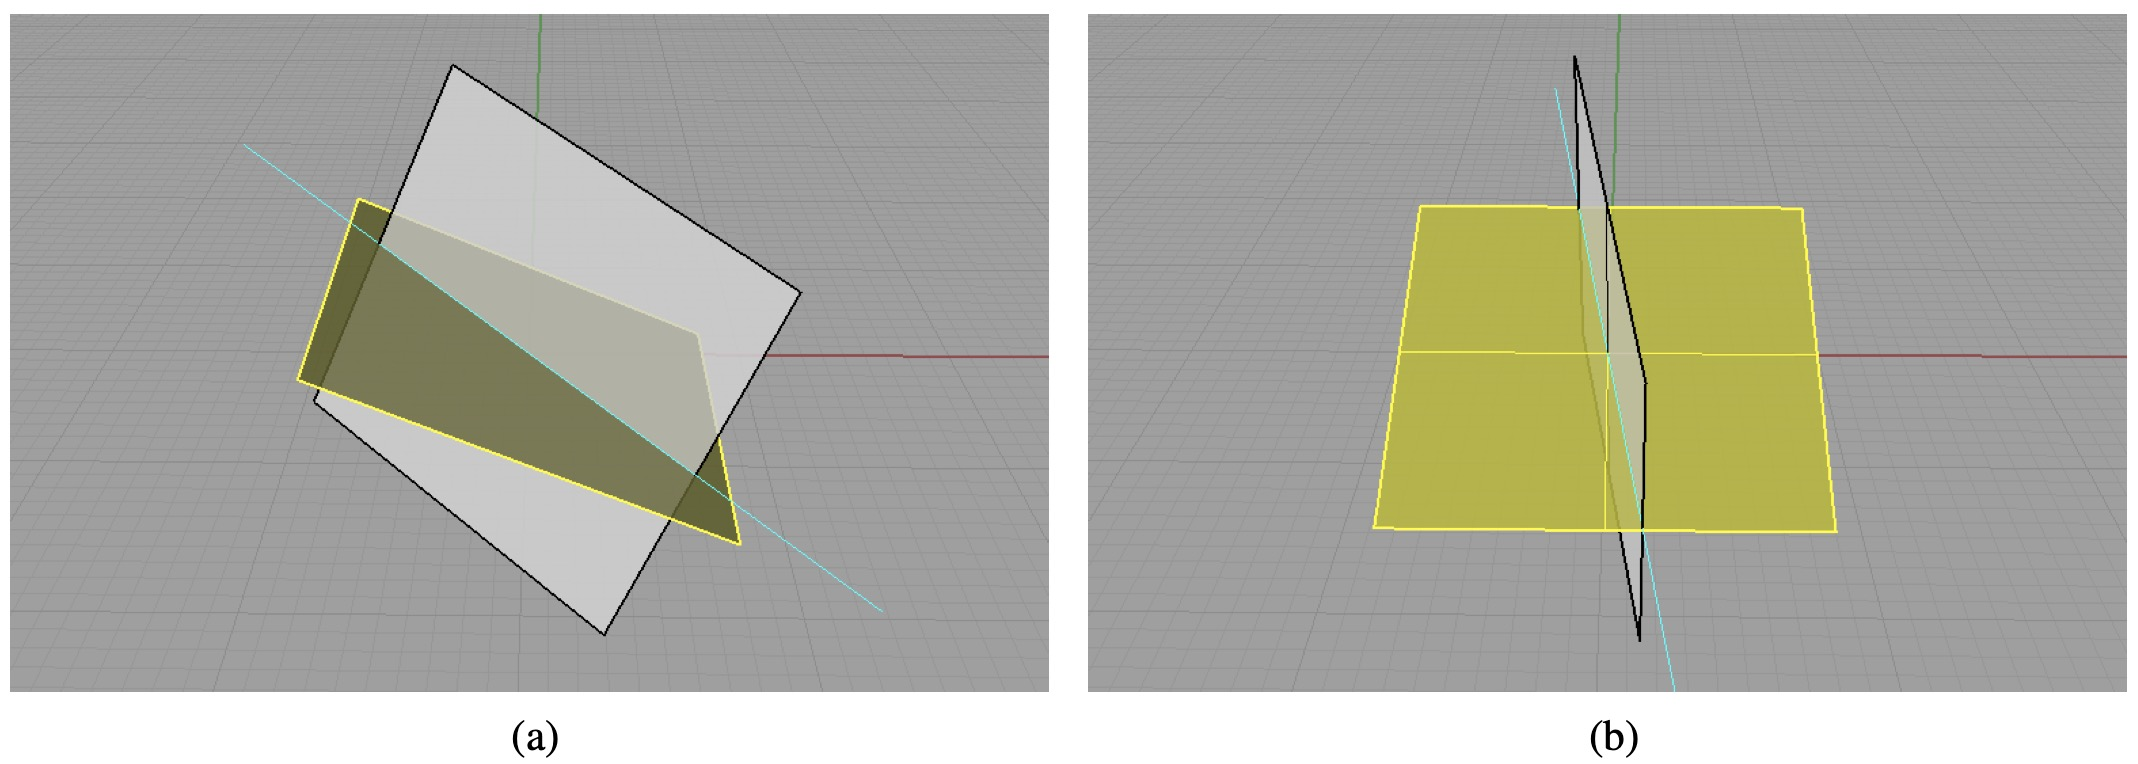
\includegraphics[width=0.5\textwidth]{pictures/ray-plane.jpg}
	\caption{The intersection-of-plane representation of a ray. If $|\mathbf{d}_x| > |\mathbf{d}_y| \mathrm{\ and\ } |\mathbf{d}_x| > |\mathbf{d}_z|$ holds, the first plane is rotated about the $z$-axis and the other plane is perpendicular to it (a). If it does not holds, the first plane is instead rotated about the $x$-axis(b)}.
	\label{fig:ray-representation}
\end{figure}

In this way, an intersection point on the surface $\mathbf{S}$ can be found by solving the following system of equations:
\[\begin{cases}
	\mathbf{P}_1 \cdot (\mathbf{S}(u, v), 1) = 0\\
	\mathbf{P}_2 \cdot (\mathbf{S}(u, v), 1) = 0
\end{cases}\]

Note that this transformation allows the intersection of the ray with the patch to be found by solving for $u$ and $v$ parameters, instead of direcly getting the intersection point information in 3D space. That's why we are ray tracing NURBS directly, which potentially saves computation time.

\subsubsection{Ray-Bezier-Patch Intersection Test}

% 这里介绍如何计算ray和bezier patch的交点(牛顿迭代法)
\ 

One of the most important part in ray tracing NURBS is to calculate intersection between a ray and a surface patch. We are going to solve this problem by \textit{Newton-Rhapson method}. The general idea is that, we start from an initial guess, and compute the tangent line to approximate the function and calculate the $x$-intercept of it. 

\begin{figure}[H]
	\centering
	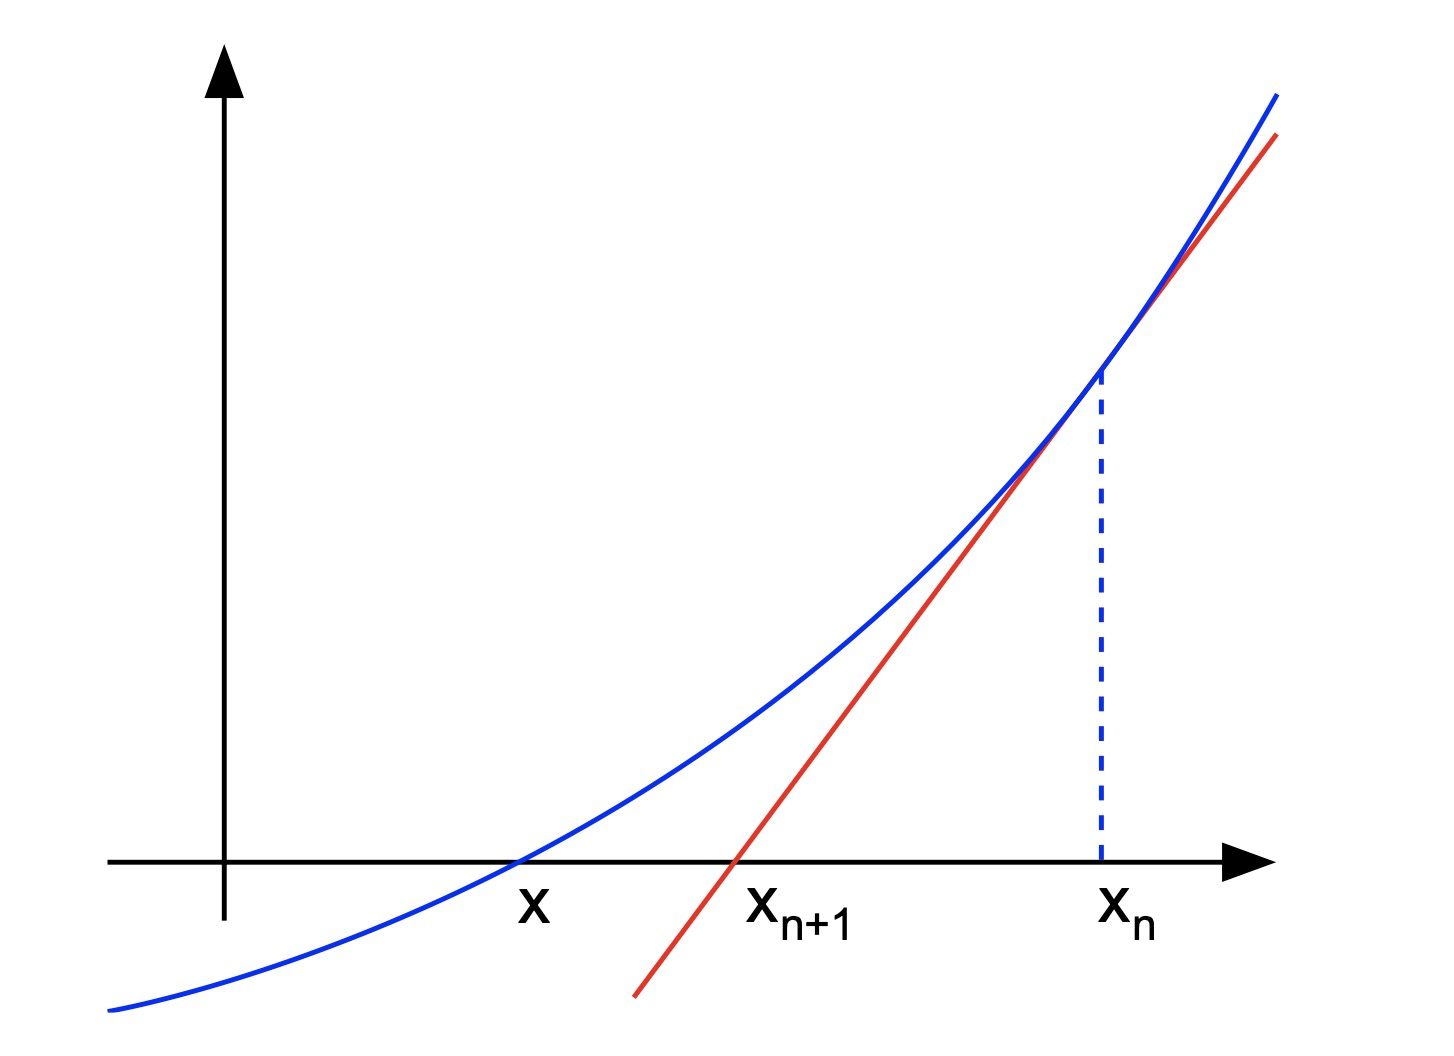
\includegraphics[width=0.3\textwidth]{pictures/newton-iteration.jpg}
	\caption{Newton-Rhapson method's iteration. The root is $x$, the original guess is $x_n$, and the new guess is $x_{n+1}$. The new guess is closer to the root.}
\end{figure}

In ray tracing NURBS, we start from an initial guess of $u$ and $v$, which is the mid point of the valid range. We iterate the following until convergence: 

\[
	\left(\begin{matrix}
		u_{n+1} \\ v_{n+1}
	\end{matrix}\right)	
	= 
	\left(\begin{matrix}
		u_n \\ v_n
	\end{matrix}\right) - 
	\left(\mathbf{J}\right)^{-1}
	\left(\begin{matrix}
		f(u_n, v_n) \\ g(u_n, v_n)
	\end{matrix}\right)
\]

The Jacobian matrix is defined as \[
	\mathbf{J} = (\mathbf{F}_u, \mathbf{F}_v)	
\] where \[
	\mathbf{F}_u = \left(\begin{matrix}
		\mathbf{N}_1 \cdot \mathbf{S}_u(u, v)\\
		\mathbf{N}_2 \cdot \mathbf{S}_u(u, v)
	\end{matrix}\right)	
\]\[
	\mathbf{F}_v = \left(\begin{matrix}
		\mathbf{N}_1 \cdot \mathbf{S}_v(u, v)\\
		\mathbf{N}_2 \cdot \mathbf{S}_v(u, v)
	\end{matrix}\right)	
\]

We use the following conditions to determine whether we should stop the Newton iteration. 

\begin{itemize}
	\item We limit the number of iterations to $7$. If no solution can be found after the max number of iteractions, we stop and return no intersection. According to \cite{}, the average number of iterations needed to produce convergence is 2 or 3 in practice, so $7$ is enough.
	
	\item If the distance to the root is nearly zero (less than a predetermined $\epsilon$ in practice), we conclude that an intersection happens. We then evaluate the intersection information (including position, normal) by the value of $u$ and $v$.
	\[
		\| \mathbf{F}(u_n, v_n) \| < \epsilon	
	\]
	Since the value of $u$, $v$ we get is approximate, it may not necessarily lie along the ray. Therefore we perform a projection along the ray direction to get the intersection point. \[
		t = (\mathbf{P} - \mathbf{o}) \cdot \mathbf{d}	
	\]

	\item We don't allow the new estimate further from the root compared with the last estimate. That is \[
		\| \mathbf{F}(u_{n+1}, v_{n+1}) \| >
		\| \mathbf{F}(u_{n}, v_{n}) \|
	\] 
	If this happens, we assume divergence, so we stop and return no intersection.

	\item We don't allow $u$ and $v$ to exceed the parametric domain of the surface. \[
		u \notin [u_{min}, u_{max}] \mathrm{\ or\ } v \notin [v_{min}, v_{max}]	
	\]
	If after some iterations, the new estimate is out of the domain, we stop and return no intersection.
\end{itemize}

After each iteration, we will also assure that the Jacobian matrix $\mathbf{J}$ is not singular before updating the new estimate. To determine its singularity, we test if \[
	\det(\mathbf{J}) = 0	
\]
If the Jacobian is singular, we iterate by the following equation
\[
	\left(\begin{matrix}
		u_{k+1}\\v_{k+1}
	\end{matrix}\right)	= 
	\left(\begin{matrix}
		u_{k}\\v_{k}
	\end{matrix}\right) + 0.1 \cdot \left(\begin{matrix}
		\mathrm{drand48}() \cdot (u_0 - u_k)\\
		\mathrm{drand48}() \cdot (v_0 - v_k)\\
	\end{matrix}\right)
\] where $\mathrm{drand48()}$ returns a random floating number between $0.0$ and $1.0$.

The pseudo code is given as follows:  

% \begin{lstlisting}[language=c++]
% \end{lstlisting}


\subsubsection{Point Derivative Evaluation}

% TODO: 这里要写如何求point (u,v)的导数,也就是论文中的2.4 Evaluation 这一章

In the above section, we need to calculate the Jacobian matrix which consists of four derivatives. We will explain how to calculate these derivatives in this part. 

\[
	\mathbf{S}(u_*, v_*) = \mathbf{D}_{\mu_u - \mathbf{k}_u + \mathbf{1}, \mu_v - \mathbf{k}_v + \mathbf{1}}	
\] 
\[\begin{aligned}
	\mathbf{S_u}(u_*, v_*) =& \frac{
		(k_u-1)\omega_{\mu_u - k_u + 2, \mu_v - k_v + 1}
	}{
		(u_{\mu_u + 1} - u_*)\omega_{\mu_u - k_u + 1, \mu_v - k_v + 1}
	}\cdot \\ &\left[
		\mathbf{D}_{\mu_u - \mathbf{k}_u + \mathbf{2}, \mu_v - \mathbf{k}_v + \mathbf{1}} - 
		\mathbf{D}_{\mu_u - \mathbf{k}_u + \mathbf{2}, \mu_v - \mathbf{k}_v + \mathbf{1}}
	\right]
\end{aligned}
\]
\[\begin{aligned}
	\mathbf{S_v}(u_*, v_*) =& \frac{
		(k_v-1)\omega_{\mu_u - k_u + 1, \mu_v - k_v + 2}
	}{
		(v_{\mu_v + 1} - v_*)\omega_{\mu_u - k_u + 1, \mu_v - k_v + 1}
	}\cdot \\ &\left[
		\mathbf{D}_{\mu_u - \mathbf{k}_u + \mathbf{1}, \mu_v - \mathbf{k}_v + \mathbf{2}} - 
		\mathbf{D}_{\mu_u - \mathbf{k}_u + \mathbf{2}, \mu_v - \mathbf{k}_v + \mathbf{1}}
	\right]
\end{aligned}
\]

\section{Results}

% TODO: bug没修完还没画出来。

\begin{figure}[H]
	\centering
	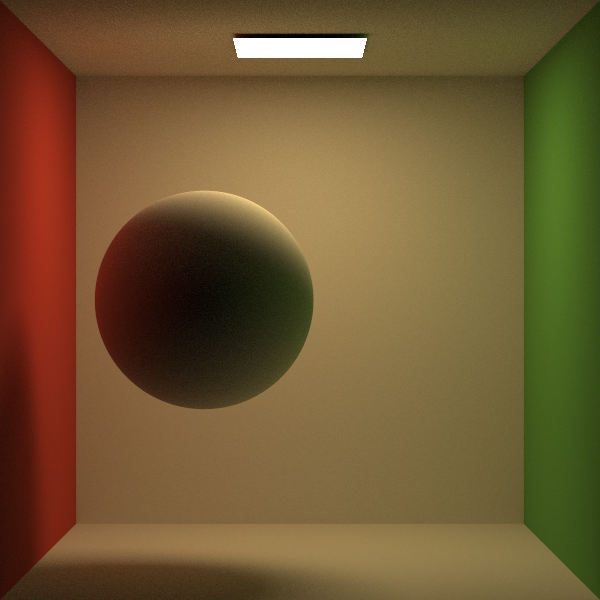
\includegraphics[width=0.4\textwidth]{results/result600.png}
	\caption{A NURBS ball}
	\label{fig:result1}
\end{figure}



\end{document}
